\defcitealias{Tarango-Yong:2018a}{Paper~I}
\newcommand\PaperI{\citetalias{Tarango-Yong:2018a}}

\section{Introduction}
\label{sec:introduction}
\newcommand\hii{\ion{H}{ii}}

Curved emission arcs around stars \citep[e.g.,][]{Gull:1979a} are
often interpreted as \textit{bow shocks}, due to a supersonic
hydrodynamic interaction between the star's wind and an external
stream. This stream may be due to the star's own motion or to an
independent flow, such as an \hii{} region in the champagne phase
\citep{Tenorio-Tagle:1979a}, or another star's wind
\citep{Canto:1996}. However, an alternative interpretation in some
cases may be a radiation-pressure driven bow wave, as first proposed
by \citet[\S\textsc{vi}]{van-Buren:1988a}.  In this scenario, photons
emitted by the star are absorbed by dust grains in the incoming
stream, with the resultant momentum transfer being sufficient to
decelerate and deflect the grains within a certain distance from the
star, forming a dust-free, bow-shaped cavity with an enhanced dust
density at its edge.  Two regimes are possible, depending on the
strength of coupling between the gas (or plasma) and the dust.  In the
strong-coupling regime, gas--grain drag decelerates the gas along with
the dust, forming a shocked gas shell in a similar fashion to the
wind-driven bow shock case.  In the weak-coupling regime, the gas
stream is relatively unaffected and the dust temporarily decouples to
form a dust-only shell.  This second case has recently been studied in
detail in the context of the interaction of late O-type stars (which
have only weak stellar winds) with dusty photoevaporation flows inside
\hii{} regions \citep{Ochsendorf:2014a, Ochsendorf:2014b,
  Ochsendorf:2015a}.  We follow the nomenclature proposed by
\citet{Ochsendorf:2014b}, in which \textit{dust wave} refers to the
weak coupling case and \textit{bow wave} to the strong coupling case.
More complex, hybrid scenarios are also possible, such as that studied
by \citet{van-Marle:2011a}, where a hydrodynamic bow shock forms, but
the larger dust grains that accompany the stellar wind pass right
through the shocked gas shell, and form their own dust wave at a
larger radius.

\begin{figure}
  \centering
  \framebox{
    \parbox[m][4cm]{0.8\linewidth}
    {\centerline{\textbf{\dotfill TODO\dotfill}}}}
  \caption{Bow shocks, bow waves, and dust waves}
  \label{fig:3-types-bow}
\end{figure}

In \citet[][hereafter \PaperI{}]{Tarango-Yong:2018a}, we proposed a
new two-dimensional classification scheme for bow shapes: the
projected planitude--alatude, or \(\Pi'\)--\(\Lambda'\), diagram.  Planitude
measures the flatness of the bow's apex, while alatude measures the
openness of the bow's wings.  Both are dimensionless ratios of lengths
that can be estimated from observational images.  We have analyzed the
inclination-dependent tracks on the \(\Pi'\)--\(\Lambda'\) plane for simple
geometric shapes (spheroids, paraboloids, hyperboloids) and for
thin-shell hydrodynamic bow shock models (wilkinoid, cantoids,
ancantoids).  In this paper, we will do the same for simple models of
radiation-driven dust waves (dragoids) and bow waves (trapoids).

The paper is organized as follows.
%
In \S~\ref{sec:shape-dust-wave} we do the same for simple models of a
dusty radiation bow wave (dragoids), including the effects of
gas-grain drag.
%
In \S~\ref{sec:perturbed-bows} we investigate the effects on the
planitude--alatude plane of small-amplitude perturbations to the bow
shape.
%


\section{Different types of bow}
\label{sec:different-types-bow}

\begin{figure*}
  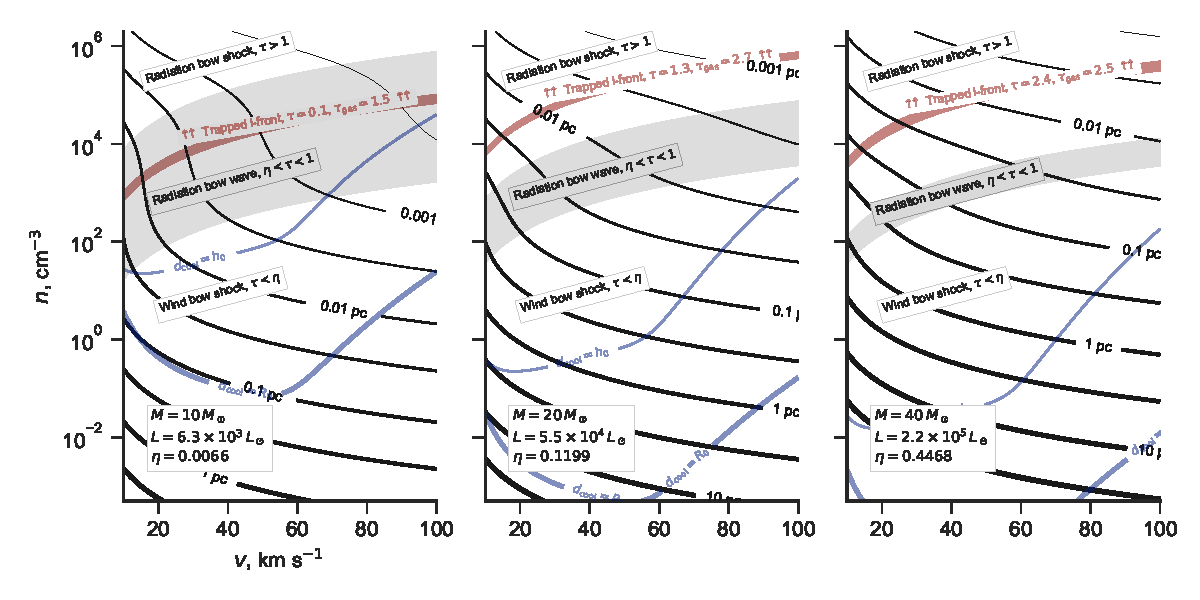
\includegraphics[width=\linewidth]{figs/zones-v-n-plane}
  \caption{Bow regimes of parameter space (\(v, n\)) of the external
    stream for main-sequence OB stars of different masses:
    (a)~\SI{10}{M_\odot}, (b)~\SI{20}{M_\odot}, (c)~\SI{40}{M_\odot}. }
  \label{fig:zones-v-n-plane}
\end{figure*}

We will mainly consider the canonical case of a bow around a star of
bolometric luminosity, \(L\), with a radiatively driven
wind,\footnote{In \S~\ref{sec:case-inside-out} we consider the case of
  an external luminous source.} which is immersed in an external
stream of gas and dust with density, \(\rho\), and velocity, \(v\).  The
size and shape of the bow is determined by a generalized balance of
pressure (or, equivalently, momentum) between internal and external
sources.  We assume that the stream is supersonic and super-alfvenic,
so that the external pressure is dominated by the ram pressure:
\(\rho v^2\).


\subsection{Imperfect coupling between gas and dust}
\label{sec:imperf-coupl-betw}

\begin{figure}
  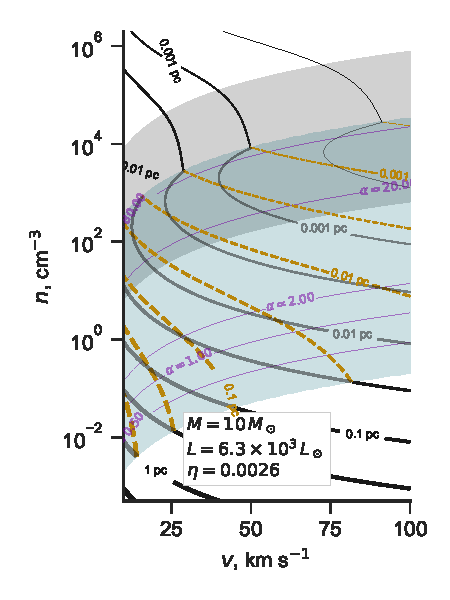
\includegraphics[width=\linewidth]{figs/decouple-v-n-plane}
  \caption{As Fig.~\ref{fig:zones-v-n-plane}(a), but accounting for
    gas-grain decoupling with constant efficiency \(\xi = 0.07\). }
  \label{fig:decouple-v-n-plane}
\end{figure}

\begin{figure}
  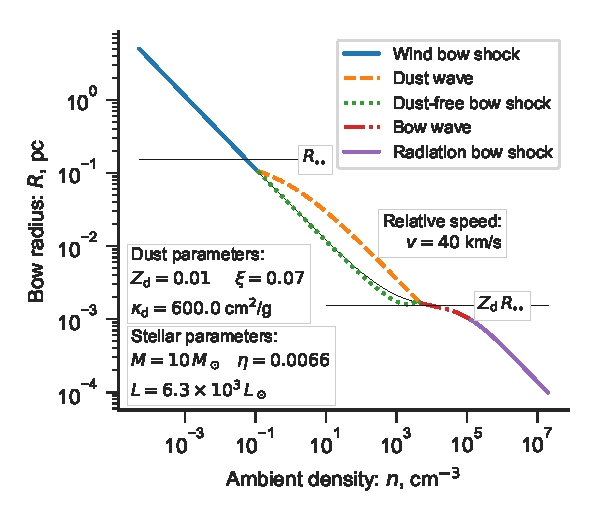
\includegraphics[width=\linewidth]{figs/decouple-v40-versus-n}
  \caption{Vertical cut through Fig.~\ref{fig:decouple-v-n-plane},
    showing bow radius and different regimes for a fixed inflow
    velocity of \SI{40}{km.s^{-1}}.}
  \label{fig:decouple-v40-versus-n}
\end{figure}


\subsection{The case of inside-out bows with external illumination}
\label{sec:case-inside-out}


%%% Local Variables:
%%% mode: latex
%%% TeX-master: "dusty-bow-wave"
%%% End:
